 \documentclass[manuscript]{aastex}

%-- Packages 
\usepackage[backref, breaklinks, colorlinks, citecolor=blue, linkcolor=magenta]{hyperref}

%\documentclass[]{emulateapj}
\newcommand{\vdag}{(v)^\dagger}
\newcommand{\myemail}{skywalker@galaxy.far.far.away}

\slugcomment{Submitted to The Astrophysical Journal}

\shorttitle{Gas Accretion in MW-like Galaxies}
\shortauthors{N. N. Sanchez, J. M. Bellovary, \& K. Holley-Bockelmann}

\usepackage{natbib}
%\bibliographystyle{plain}
\bibliographystyle{apj}

\begin{document} 

\title{A Particular Appetite: Cosmological Hydrodynamic Simulations of Preferential Accretion in the Supermassive Black Holes of Milky Way Size Galaxies}



\author{N. Nicole Sanchez \altaffilmark{1, 2}}
\author{Jillian M. Bellovary\altaffilmark{1, 2, 3}}
\author{Kelly Holley-Bockelmann\altaffilmark{1, 2}}

\affil{$^1$Fisk University, Nashville, TN, USA, n.nicole.sanchez@vanderbilt.edu}
\affil{$^2$Vanderbilt University, Nashville, TN, USA}
\affil{$^3$American Museum of Natural History, New York, NY, USA}


\begin{abstract}\label{abs:abstractlabel}

[IAU Abstract as Placeholder] Using cosmological hydrodynamic simulations of Milky Way-type Galaxies, we explore the effect of accreted gas as feeding mechanisms for supermassive black holes. By examining two of these galaxies with differing merger histories, one characterized by several major mergers and the other with a quiescent history, we can examine the importance of merger history on black hole accretion. This study is an extension of Bellovary et. al. 2013, which did a similar study analyzing the accretion of high mass, high redshift galaxies and their central black holes. Bellovary found that the gas accreted by the central black holes was proportional to that accreted by the host galaxy. Contrary to the previous study's results, we've found that while a galaxy with a quiescent history will still have a black hole mirroring the accretion of its host, a galaxy with an active merger history has a central black hole that is preferentially fueled by gas accreted through mergers. We look to the the angular momentum of the accreted gas in these Milky Way analogs to develop a clearer picture of the mechanisms best fueling their central SMBHs.

\end{abstract}

\keywords{Black hole physics -- Galaxies: spiral -- Galaxies: kinematics and dynamics -- Methods: Numerical -- Others?}

\section{Introduction}\label{sec-intro}

[Note to self: Cite one canonical person but also more junior people in the field.]

\citep[for example; ][at the end of the line]{Bellovary2010,Tremmel2015,Fu2008}


 \S\ref{sec-intro}


Supermassive black holes (SMBHs) are thought to exist in almost all massive galaxies. \citep{Kormendy2013} [OTHERS?] In the canonical picture of BH growth, these black holes may become active galactic nuclei (AGN) during periods of high accretion and wane in periods of quiescence. \citep{Volonteri2012} [GET OBS REFS] The host galaxy's size, star formation rate, and other environmental effects may help to influence the growth of the black hole residing at its center [REFS]; however, there are still uncertainties concerning the relationship between these SMBHs and their much larger host galaxies, as well as how they grow and evolve together. [ADD REFS FROM REVIEWS; + \citep{Fu2008}]

[Note to self: Make sure paper thoroughly discusses what we think we KNOW about growth/evolution and what is still being DEBATED]

The M$-\sigma$ relation, which relates the SMBH's mass and the velocity dispersion of the host galaxy's central stellar population, gives some insight into the complex interplay between these objects. \citep{Kormendy2013} A prominent trend appears, as SMBHs tend to scale with the velocity dispersion of the host galaxy bulge. % For my thesis: A prominent trend appears as SMBHs tend to scale with the spheroidal center of their host galaxies; i.e. less massive SMBH reside in galaxies with less disperse bulges, and more massive SMBH live in galaxies with larger velocity dispersions in their bulges. 
The tightness of the relation is significant and can be seen over several orders of magnitudes in velocity dispersion and black hole mass. (\cite{Mcconnell2013}; \cite{Kormendy2013}; \cite{Merritt2001}) Scatter exists among the low mass galaxies and a deviation may appear at the high mass end, where over massive BHs may reside. [Vanden Bosch, Emsellem, Prija, maybe Volonteri?] However, scatter in less massive galaxies may imply that there are several channels of black hole growth at play in the low mass end of the relation. [Micic, previous Kelly student (ask Kelly, couldnt read this word), Volonteri] One standard explanation for the M$-\sigma$ relation lies in galaxy mergers, which build up galaxies, feed SMBHs, and assemble bulges. [Mick and others] These large, active mergers are thought to create feedback from the SMBH which affects the structure of the galaxy. [REFS]

%McConnell and Ma have the prettiest M-sigma relation, but there are two camps: Kormendy and Ferrarese & Merritt who must both be cited.
%Check with Kelly: Which Vanden, Bosch, Emsellem, and Prija papers she would recommend.


[CITE FOR THEORY: Springel and Dimatteo; cite when we discuss why m-sigma happens]

% For thesis: M-sigma plot:
%\begin{figure}
%\centerline{\resizebox{0.75\hsize}{!}{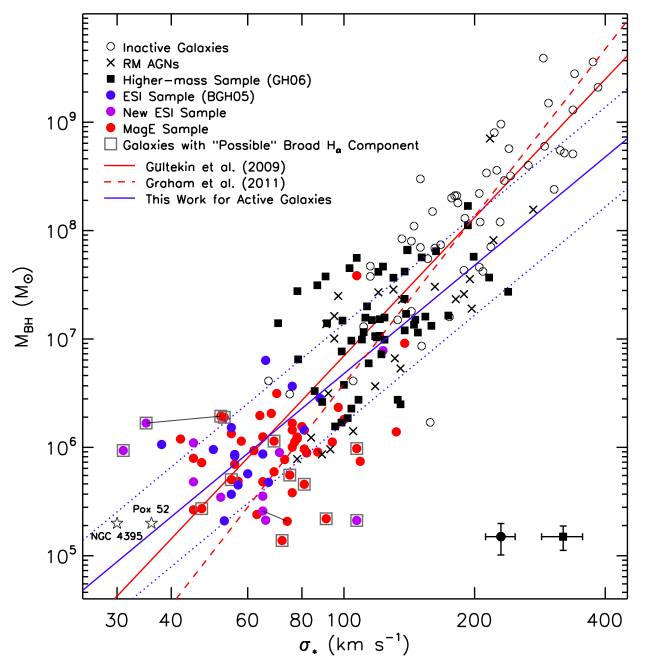
\includegraphics[angle=0]{fancymsigma}}}
%\caption[]{Gas fraction across redshift for galaxy (solid lines) and central BH (dashed lines). Green lines signify gas fractions accreted via mergers and blue lines designate gas accreted via cold flow.}
%\label{msigma} 
%\end{figure}
% Cite: Xiao

% For thesis: Explain feedback:
%Black hole feedback: the reaction effect of the energy obtained through gas accretion, which affects the overarching structure of the host galaxy.

The M$_{BH}$-bulge luminosity relation was first implied by the work of Dressler \& Richstone 1988 and Dressler 1989 first proposed the correlation while it was first illustrated by Kormendy 1993a. The M$_{BH}$-bulge mass relation followed and was determined via ground based observations by Magorrian 1998 and was around M$_{BH}$ ~ 0.005 M$_{bulge}$; however, this relation was characterized by a lot of scatter and its reliability waned due to selection biases.  Follow up examinations by others using HST observations constrained the M$_{BH}$/M$_{bulge}$ fraction to between about 0.0013 and 0.0023 (Merritt \& Ferrarese 2001; cf. McLure \& Dunlop 2002 and Marconi \& Hunt 2003, respectively). 

Major mergers between massive galaxies are thought to be efficient fueling mechanisms for bright AGN. The large influx of material due to tidal torques from the merger cause bursts of star formation and helps funnel gas directly into the center where the SMBH resides. (Hopkins 2010 canonical on tidal torques/ang mom, Richards 06, Reddy 08) Additionally, the most massive, highest-luminosity AGN (i.e. quasars) reside in incredibly luminous infrared galaxies where star formation is abundant, signifying that major mergers may have recently occurred. [REFS] Distorted morphologies are often characteristics of quasar hosts, and companions can also be present around quasars, both of which are evidence that strengthen the possibility of a recent merger having affected their lifetimes. [REFS] 

	In many less massive AGN [REFS], however, there is a clear lack of distorted morphologies, close neighbors, and/or other obvious merger evidence.  [Ryan 2007 (Seyfert 1, smaller than MWG), Hicks 2013 (Seyfert and quiescent galaxies)]  It is also important to note that many of these AGN exist in spiral galaxies, which are unlikely to have been recently disturbed by major mergers. (Schawinski 2011; Kocevski 2012) Nevertheless, some evidence suggests (Governato 2009) that disturbed galaxies may reform a disk quickly, even if their history is characterized by many mergers. More recently, Triester (2012) has suggested that only the highest luminosity AGN require fueling via major mergers, an effect which seems to scale with luminosity rather than redshift. They found that ~90\% of AGN across all redshifts are fueled by various other mechanisms which may include minor mergers, flybys, and smooth accretion, whereby gas is directly accreted via large filaments from the ambient intergalactic medium. Secular processes, including bar formation and disk instabilities, may also be prominent forms of accretion for these SMBHs. [REFS; maybe Graham, or K\& Ho]  

	Smooth accretion of cold flow gas seems a likely candidate for fueling these low mass galaxies. Filaments of unshocked gas may fuel until the galaxy halo reaches a total (virial) mass near 10$^{11} M_{\odot}$ [DiMatteo(maybe), Keres 05, Brooks 2007; maybe Dekel (look at who cites Keres and Brooks in ADS]; once in more massive halos, the gas will shock heat to the virial temperature of the halo.  % For my thesis: The cold flow filaments that feed thses galaxies are dependent on the galaxy's mass. Smoothly accreted gas will fuel through cold flow filaments until the galaxy halo reaches a a mass near 10$^{11} M_{\odot}$. Once the galaxy's mass is greater than this threshold, the mass will reach the virial radius of the halo and the rapid increase in temperature within the radius causes the gas to shock as its temperature quickly increases.



It is known that galaxy hosts grow through different channels that depend on mass, environment, and interaction history; therefore, we would like to understand how these different galaxy evolutionary paths translate into different SMBH fueling mechanisms, and to see if it affects the state of fueling gas flowing into the SMBH itself. Therefore, we will also discuss the fueling mechanisms which also vary between galaxies of similar mass due to different merger and formation histories.
	
	 In this paper, we discuss the gas accretion history within two galaxy simulations that appear similar at z = 0 but have very different merger histories. Our "active" galaxy, h258, has a history characterized by many major mergers, while our "quiet" galaxy, h277, has a quiescent history dominated by cold flow accretion and few minor mergers. These galaxies look quite similar at z=0, and have many of the same properties as the Milky Way including M$_{vir}$ (mass within the virial radius), stellar mass, and v$_{circ}$ (circular velocity). However, without a deeper examination, we might not realize they have such varying merger histories. Milky Way-type galaxies host SMBHs on the order of 10$^6$ M, which are likely the most common type of massive black hole, yet little is known about them or how they may grow. By examining the feeding mechanisms of these galaxies, as well as what type of gas feeds their central SMBHs, we will be able to compare the accretion rates between h258 and h277 to determine which accretion methods dominate within the central regions of these Milky Way-size galaxies. 
	
	\cite{Bellovary2013} compared simulations of three high mass, high redshift galaxies and found that while mergers and smooth accretion both build up galaxies, no particular method was more adept at feeding the SMBH at their centers. Using a similar method as \cite{Bellovary2013}, this work compares the fueling mechanisms between two MW mass galaxies and the accretion affecting each of their SMBHs. We will compare the BH fractions and halo fractions between and within the galaxies to look for clues about SMBH preferential feeding within these MW-size galaxies and how their histories lead to galaxies with such similar structure.
	
	
	
	
	
	
  
\section{Simulation Parameters}\label{sec-model}

\subsection{Low Resolution GASOLINE Simulations}

	The cosmological simulations have been run using the smoothed particle hydrodynamics (SPH) N-body tree code Gasoline (Stadel 2001; Wadsley 2004). \citep{Wadsley2004} Prescriptions for star formation, supernova feedback (Stinson 2006), metal diffusion (Shen 2010), and MBH formation, feedback, and accretion \citep{Bellovary2010} are included within Gasoline. Each simulations assumes a WMAP cosmological model (Spergel 2007), Kroupa initial mass function (Kroupa 2001), and a uniformly distributed ultraviolet background (Haardt \& Madau 1996). Gasoline simulated galaxies are shown to lie conform with the observed Tully-Fisher relation (Governato 2009), the size-luminosity relation (Brooks 2011), and the mass-metallicity relation (Brooks 2007), in addition to having realistic matter distributions and baryon fractions (Governato 2010; Guedes 2011). Primordial cooling and a low-temperature extension to the cooling curve is used to trace metals (Bromm2001). Gas is allowed to reach a minimum temperature of ~100 K, though cooling via molecular hydrogen or metals is not included. The aforementioned works have previously demonstrated that realistic galaxy models can be obtained without the use of these advanced features. (Christensen2012, in addition). Though these previous works have not included AGN feedback or its effects, for small to moderate mass galaxies (like those of previous and current studies) our research shows their central supermassive black holes have little affect on the global properties of their hosts and only directly impacts the central region of their galaxy. Therefore, we are confident these simulations are in good accordance with the broad range of properties in current galaxy observations.

	We have examined two simulations, each of a uniform volume cube with 50 Mpc sides. [Volume normalization technique?] The main halo of each simulation results in a Milky Way-size spiral galaxies with z=0 masses between 6--8 $\times$ 10$^{11}$  M$_{\odot}$. The simulations each have a force resolution of 300 pc [Note: I have 300 written in my research notebook, but B13 says 260. The notes I have are the ones I took so AAS so maybe that's a rounded up value?]. The gas, dark matter, and star particles have masses of 2 $\times$ 10$^5$ M$_{\odot}$, 3 $\times$ 10$^5$ M$_{\odot}$, and 7 $\times$ 10$^4$ M$_{\odot}$, respectively.  [Jillian's paper includes a table of simulation properties. Should I create one as well? I feel like yes.] 

	The simulation includes stochastically modeled star formation, including a density threshold (2.5 amu cm$^-3$) for gas particles above which they become eligible to form stars; the gas must also be below a temperature threshold of 10$^4$ K. Additionally, we utilize a star formation efficiency parameter of c$^*$ $=$ 0.1. Our supernova feedback energy is E$_SN$ $=$ 1 $\times$ 10$^51$ erg and, using the blastwave equations from McKee \& Ostriker (1977), the energy is passed to surrounding particles within a calculated radius. The equation also determine how long the cooling is shut off for heated particles. These parameters and resolution choice allow the galaxies to adhere to the stellar-mass-halo-mass relation at z=0 and maintain a realistic period of star formation. (Moster 2010; Munshi 2013) We are confident with these criteria and restraints that we reasonably represent growth in the galaxy and its SMBH. [Note: I did change the variables to h258/h277 values. Cstar is the same, but Esn was larger.]

	%Like the star formation, seed black hole formation is modeled stochastically but requires the additional stipulation that black holes must form from zero-metallicity gas. A gas particle that has zero-metallicity and also meets the requirements for star formation will have a probability, $\chi_{seed}$, that it will become a black hole. The resulting black hole will maintain the same mass as its parent gas particle (2 $\times$ 10$^5$) M$_{\odot}$. We set  $\chi_{seed}$ $=$ 0.1 to achieve adequate MBH occupation fractions, without an over production of merger events between MBHs. This circumvents the Soltan arguments wherein mergers alone feed MBHs almost entirely without allowing for accretion growth. This method is nearly consistent the theories of direct collapse black holes from gas (Couchmann \& Rees 1986, Abel 2002, Bromm \& Larson 2004) and Population III star black hole formation (Loeb \& Rasio 1994, Eisentstein \& Loeb 1995, Koushiappas 2004, Begelmann 2006, Lodato \& Natarajan 2006). Utilizing this requirement, we ensure that black hole formation ceases at high redshift, since at this time the interstellar medium (ISM) has become overwhelmed with metals due to supernova remnants. Black holes are not fixed within their host, allowing them to be dynamically affected by mergers and other perturbations within the galaxy.  Multiples may also form within the same halo. Dark matter particles have slightly larger masses than black holes to tamper the effects of artificial two-body scattering and to keep the black holes in the center of their dark matter host particles. \\

	%There are still many uncertainties regarding the formation of black holes "seeds" and their evolution into the SMBHs we see at the centers of galaxies. Neverthless, we do know there must be some method driving their quick transformation from seeds to quasars that can be seen at z ~ 6. [Fan 2001] We assume the method of direct collapse from pristine, low metallicity gas to create our seed BHs. [Begelman 2006] While this method allows the BH formation process to remain physically motivated, the choice of BH seeding method is not terribly important as our focus remains on the dynamic evolution of the seeds, which is not dependent on their initial mass (10$^5$ M$_{\odot}$ for the direct collapse scenario and 100 M$_{\odot}$ for the first stars [Include latter half of sentence? Is that method used?]). These heavier BH seeds have a dynamical friction time longer than the Hubble time, due to local densities. BH seeds form if their parent gas particle match the criteria required for star formation] and also maintain zero metallicity. [Stinson 2006 for star formation details] A probability of $\chi_{seed}$ = 0.01 is applied to determine whether a gas particle (with the above specifications) will become a BH seed with a mass of M$_{BH}$ = 2.28 $\times$ 10$^5$ M$_{\odot}$, the same mass as its parent gas particle. This probability was chosen to match the predicted occupation probability of BH seeds at z ~ 3. [Volonteri 2008] BH seed formation ends at z ~ 3.5 due to the dilution of pristine gas by efficient metal diffusion expected after the first population of supernovae. The requirement that BH seeds must form from zero metallicity gas particles also causes BH formation to be constrained in areas of early star formation bursts, where the earliest and most massive halos are expected to form in the simulation. Should two BHs form within a softening length, the BHs merge into one with a mass equal to the sum of both BH seed masses. BHs formation is dependent only on their local environment, neglecting any large-scale properties of the host halo. BHs are also allowed to move within their halos, if influenced by external forces, rather than being artificially pinned to the centers of their host halos. Nevertheless, BHs are kept near their host centers by choosing dark matter particles masses in high-resolution regions to be on the same order as gas particle masses which minimizes two-body interactions. [Bellovary et. al. 2010]\\
	

	There are still many uncertainties regarding the formation of black holes "seeds" and their evolution into the SMBHs we see at the centers of galaxies. Neverthless, we do know there must be some method driving their quick transformation from seeds to quasars that can be seen at z ~ 6. [Fan 2001] We assume the method of direct collapse from pristine, low metallicity gas to create our seed BHs. [Begelman 2006] While this method allows the BH formation process to remain physically motivated, the choice of BH seeding method is not terribly important as our focus remains on the dynamic evolution of the seeds, which is not dependent on their initial mass (10$^5$ M$_{\odot}$ for the direct collapse scenario and 100 M$_{\odot}$ for the first stars [Include latter half of sentence? Is that method used?]). These heavier BH seeds have a dynamical friction time longer than the Hubble time, due to local densities. BH seeds form if their parent gas particle match the criteria required for star formation] and also maintain zero metallicity. [Stinson 2006 for star formation details] A probability of $\chi_{seed}$ = 0.01 is applied to determine whether a gas particle (with the above specifications) will become a BH seed with a mass of M$_{BH}$ = 2.28 $\times$ 10$^5$ M$_{\odot}$, the same mass as its parent gas particle. This probability was chosen to match the predicted occupation probability of BH seeds at z ~ 3. [Volonteri 2008] This circumvents the Soltan arguments wherein mergers alone feed BHs almost entirely without allowing for accretion growth. This method is nearly consistent the theories of direct collapse black holes from gas (Couchmann \& Rees 1986, Abel 2002, Bromm \& Larson 2004) and Population III star black hole formation (Loeb \& Rasio 1994, Eisentstein \& Loeb 1995, Koushiappas 2004, Begelmann 2006, Lodato \& Natarajan 2006). BH seed formation ends at z ~ 3.5 due to the dilution of pristine gas by efficient metal diffusion expected after the first population of supernovae. The requirement that BH seeds must form from zero metallicity gas particles also causes BH formation to be constrained in areas of early star formation bursts, where the earliest and most massive halos are expected to form in the simulation. Should two BHs form within a softening length, the BHs merge into one with a mass equal to the sum of both BH seed masses. BHs formation is dependent only on their local environment, neglecting any large-scale properties of the host halo. Black holes are not fixed within their host, allowing them to be dynamically affected by mergers and other perturbations within the galaxy. Nevertheless, BHs are kept near their host centers by choosing dark matter particles masses in high-resolution regions to be on the same order as gas particle masses which minimizes two-body interactions. [Zolotov 2012, Bellovary et. al. 2010 for all of paragraph]

	Black hole mergers can occur when they meet two criteria. First, the black holes must be within twice the softening length of each, and they must also satisfy $(1/2) \delta v^2 < \delta a \cdot \delta r$,  where $\delta v$ and $\delta a$ are the velocity and acceleration differences between the two black holes and $\delta r$ is the distance separating them. In addition to gaining mass via merger, black holes may also accrete gas via the Bondi-Hoyle method:
\begin{equation}
\dot{M} = \frac{4 \pi \alpha G^2 M^{2}_{BH} \rho}{(c^{2}_{s} + v^2)^{3/2}},
\end{equation}

where $\alpha$ is a constant of 1, $\rho$ is the density of the surrounding gas, $c_s$ is the sound speed, and $v$ is the black hole's relative velocity compared to the gas. In response to the accretion of gas, feedback energy is released onto the surrounding gas:
\begin{equation}
\dot{E} = \epsilon _{r} \epsilon _{f} \dot{M} c^2 
\end{equation}

which is proportional to the accretion rate of gas and assumes $\epsilon _r = 0.1$ and $\epsilon _f = 0.03$ for the radiative efficiency. The efficiency $\epsilon _f = 0.03$ is where the feedback energy couples to gas, "which is distributed over the SPH kernel as thermal energy to the 32" nearest gas particles. [Look into this. Confused.] Though other groups (such as Sijacki,2007, Di Matteo 2008) use a higher value for this efficiency, $\epsilon _f = 0.05$, we've found this increased efficiency overpowers the feedback and highly limits gas accretion. Using $\epsilon _f = 0.03$, the MBHs are in better agreement with the MBH-host galaxy scaling relations, e.g. M$_{BH}$-$\sigma$ and M$_{BH}$-M$_{bulge}$. This efficiency value is a simulation parameter used in subgrid feedback models, but does not represent a specific physical quantity, and therefore some variation among codes is expected. Finally, as this work's main concern is the relative accumulation of gas through various accretion methods and not the total value of accreted gas mass, these results are not highly sensitive to adjustments in the feedback implementation.

\subsection{High Resolution CHANGA Simulations}

	Charm N-body GrAvity solver, ChaNGa, was used to run the second iteration of these N-body + SPH galaxy simulations. An initial DM-only, uniform resolution 50 comoving Mpc box was used to determine which halos would be selected for zoom-in examination, including the two halos examined in this paper. The DM-only simulation assumed a WMAP Year 3 cosmology (Spergel 2007) with the following specifications: $\Omega _m$ = 0.24, $\Omega _{\Lambda}$ = 0.76, $H_0$ = 73 km/s, and $\sigma _8$ = 0.77. The halos h258 and h277  were chosen for their Milky Way-mass at z=0 and their active and quiescent merger histories, respectively. The halos have virial masses defined relative to a critical density, $\rho _c$, where $\rho / \rho _c$ = 100 (Gross 1997) where h258 and h277 have virial masses of $M_{vir} = 7 \times 10^{11} M_\odot$ and $M_{vir} = 8 \times 10^{11} M_\odot$, respectively. A recent binary merger characterizes the h258 halo at z=1, while h277 has its last major merger near z ~ 3. A second "zoom-in" high resolution simulation was run for both of these galaxies including gas and star particles using the volume renormalization of Katz \& White 1993. This technique retains the large volume simulation size at lower resolution while allowing for only the closest few virial radii from the primary halo to be simulated at the highest resolution. By keeping the largest volumes at low resolution, we are able to account for building of angular momentum through the large scale tidal field in tidal torque theory. These high resolution simulations were run from z=150 to z=0.

	Both N-body+SPH volume renormalized simulations of h258 and h277 have been previously examined in other publications. Governato et. al. 2009 studied the regrowth of the large disk structure in h258 by z=0 when such a recent merger affects the galaxy. However, the results from Governato 2009 were based upon the previous Gasoline results described above. The results of this paper, both from Gasoline and ChaNGa, utilize the same initial conditions but the latter is simulated at a high resolution allowing the following new physics to be included:\\
	$\bullet$ spline force softening lengths of 174 pc\\
	$\bullet$ dark matter particles with masses of $1.3 \times 10^5 M_\odot$\\
	$\bullet$ initial gas particle masses of $2.7 \times 10^4 M_\odot$\\
	$\bullet$ star particles are created with 30\% of their parent gas particle mass; therefore, a maximum initial mass of 8100 $M_{\odot}$\\
	$\bullet$ star particles may lose mass through SNe an stellar winds\\
	$\bullet$ each galaxy contains about 5 million DM particles inside the virial radius at z=0 \\
	$\bullet$ each galaxy contains over 14 million DM, star, and gas particles total.\\
	
	The resolution of both force and mass in these simulations is comparable to the "Eris" simulation which has one of the highest resolutions for an N-body+SPH cosmological simulation of a Milky Way-mass galaxy so far produced.  While cooling physics and energy feedback from supernova are included in the same way as previous Gasoline simulations, these ChaNGa simulations also take into account metal line cooling and $H_2$. The high resoluation of the simulations allow for resolving the high density regions where star formation occurs at $\rho$ = 100 amu/$cm^3$ and adjusting the gas cooling and stellar formation prescriptions. By including metal line cooling, more gas is allowed to cool and fuel star formation within the central regions of the galaxy. (Christensen >2011) The new simulations also allow star formation to be directly affected by nearby $H_2$ abundances. This abundance is regulated by the gas's ability to self shield and its metallicity, characteristics inkeeping with observational results. (Leroy 2008, Bigiel 2008, Blanc 2009, Bigiel 2010, Schruba 2011) The $H_2$ prescription includes gas-phase and dust grain formation, as well as $H_2$ destruction via Lyman-Werner radiation due to nearby stars. Prior to implementing the $H_2$ model, gas particles needed to reach a density threshold while remaining below a set temperature (T < 1000 K) before star formation could occur. Utilizing the $H_2$ prescription removes the need for a density threshold as high densities ensuring stars only form in high density regions. For more details on the $H_2$ prescription, see Christensen et. al. 2012. 

	Primordial and metal-line cooling are described in Shen et. al. 2010, and also takes into account the diffusion of metals mixing in the interstellar medium. At z=9, a uniform UV background is applied to simulate the cosmic reionization energy in a variation of Haardt \& Madau 2001. Star particles form along the Kroupa initial mass function (Kroupa 1993). Supernova feedback releases $10^51$ ergs of thermal energy and affects a "blastwave" radius determined by the method of Ostriker \& McKee 1988. In the affected region, cooling turns off for a time relative to the expansion phase of the SN remnant. SN Ia and II from Thielemann 1986 and Woosley \& Weaver are adopted, respectively, and implemented through the method of Raiteri 1996. Both supernova "blastwave" radius calculations and supernova (Ia and II) prescriptions are as described in detail by Stinson 2006. These methods have proven to adhere to the observed, redshift dependent stellar mass-metallicity relation for galaxies. (Brooks 2007; Maiolino 2008)

	In this paper, we [demonstrate that these high resolution ChaNGa simulations have mirroring results to their low resolution Gasoline simulations. This second wave analysis allows us to feel confident in our results as we describe the varying accretion preferences for these simulated Milky Way-mass galaxies, h258 and h277.
	

\section{Reduction Method}\label{redux}

	
	The Amiga Halo Finder identifies all of the galaxies in the simulations by identifying the virial radii of the halos based on an overdensity using the criterion for a flat universe. (Amiga Halo Finder paper REF] We select the primary halo by determining the most massive galaxy at z=0 and locating the central SMBH. 

	In this analysis, we use the method utilized in \cite{Brooks2009} to trace gas particles from their origin, through their journey into the galaxy, and determine their position within the SMBH or its host. \cite{Brooks2009} studied the accretion of gas by galaxies in cosmological simulations with a focus on gaseous and stellar buildup of their disks. We use this method to trace the gas particles from their initial location to their moment of halo entry and, for some of the particles, into the SMBH. Utilizing this specific method allows us to determine the state of the gas as it enters the galaxy, by determining the method by which it enters the primary galaxy. By determining the method of entry, we can better track the "types of gas" fueling the SMBH resevoir. \\
	
[Kelly question: If the fingerprint of the fuel inflow is unique, can the angiular momentum of the gas infer spin?]
	
	We then trace the SMBH back through time, determining its host halo in each snapshot. Gas particles that are part of merger events are traced back through every merger they've encountered--within their merger trees--to determine their origin and which other halos each gas particles previously inhabited (Too anthropomorphic?). \\

	As we discussed in the introduction, there are a variety of fueling mechanisms thought to grow SMBH. Gas particles are initially traced prior to their accretion onto the main halo to determine whether they occupied a different halo at their formation. The particles are then classified by their method of entrance into the primary halo. If the gas particles existed in the primary halo at the first time step (z=4 in this study), they are classified as "early" gas. Gas that belonged to a different halo than the primary prior to accretion is classified as "clumpy" and enters the primary halo through mergers. All other gas is classified as entering the halo via "smooth" accretion, and is then subdivided into two categories: "cold" and "shocked." In the cases where a shock does not develop, cold gas will usually flow into the halo via large-scale, dark matter filaments. (Bellovary 2013) It's possible for the filaments to also be dense enough to pierce an already developed shock allowing for cold gas to funnel into the galaxy core where it can accrete onto the SMBH without being heated to the virial temperature.\\

	As previously described, if the galaxy halo is around or greater than 10$^{11}$ M$_{\odot} $, the gas will shock. We determine shocked particles through an increase in entropy and temperature using the following criteria:
\begin{equation}
T_{shock} \geq 3/8 T_{vir}
\end{equation}
where T$_{vir}$ is the virial temperature of the halo and T$_{shock}$ is the temperature of the gas particle, and 
\begin{equation}
\Delta S \geq S_{shock} - S_0
\end{equation}
where S$_0$ is the initial entropy of the gas particle and 
\begin{equation}
S_{shock} = log_{10}[3/8 T_{vir}^{1.5}/4 \rho_0]
\end{equation}
where $\rho_0$ is the gas density prior to experiencing the shock. The galaxies in this study reach final masses on the order of 10$^{12}$ M$_{\odot} $, therefore, shocked gas begins to enter the galaxy by the later timesteps of our simulation when it has reached this critical mass. \\

% [REPEAT] Gas entering the halo via smooth accretion, whether cold or shocked, is traced to 0.1 R$_{vir}$ from the galaxy, a distance after which the thermal status of the particle can no longer be confidently tracked, as supernova feedback can mimic virial shocking. Gas particles that reach this distance with the above increased in entropy and density are considered shocked particles, while all others are categorized as cold. ("See Brooks et. al. 2009 for complete details about shock physics.")\\

Once all the gas particles have been individually categorized, we can use these labels to determine the methods of accretion onto these Milky Way-size galaxies. With the information about which particles are accreting onto the SMBH (from the gas reservoir of particles that have been accreted by the galaxy), we can better compare the methods feeding both the galaxy and its SMBH. We can then determine whether there exists a method more efficiently building up these kinds of galaxies and their SMBH..\\

\section{Results} \label{results}

From the initial analysis of the low resolution Gasoline simulations, we have determined that the merger histories of these two galaxies has a pronounced effect on the resulting accretion of gas into the SMBH and its host. 

\subsection{Low Resolution h258: Resolution Test}
	
	The galaxy, h258, is characterized by an active merger history including a major merger at z=1. Our study found that nearly 65 \% of the gas accreted by the central SMBH was gas accreted via mergers, while only 39 \% of the total gas accreted by the galaxies was through mergers. (Figure \ref{h258piefrac}) This results shows explicitly that a preference exists for the SMBH to accrete gas gained through mergers. This is contrary to previous results of \cite{Bellovary2013}. \citep{Bellovary2013} found a \textit{slight} preference for gas of a lower angular momentum to enter the SMBH By examining the angular momentum of the gas accreted onto the SMBH at the moment it enters the halo, we were able to determine that a significant preference exists for gas with lower angular momentum to enter the SMBH. The gas attained through mergers tends to enter the halo with a lower angular momentum; this may explain the SMBH's preference for merger gas. \\


\subsection{Low Resolution h277: Resolution Test}
	
	Our quiescent galaxy, h277, was characterized by few mergers in its past, its final major merger occuring around z~3. Similar to Bellovary et. al. 2013 study, which found SMBH accretion in high mass, high redshift galaxies mirror their hosts in terms of accretion, h277's SMBH accretes a similar fraction of each type of gas, comparable to its host galaxy. (Figure \ref{h277piefrac}) So, h277, unlike the active h258, found no preference for the SMBH to prefer any one kind of gas in its accretion. Like the SMBH in the previous study, the same fraction of gas entering the halo would then be accreted onto the SMBH. (The gas enters a sort of reservoir and enters the SMBH somewhat uniformly.)  As these SMBHs are similar in size and appearance at z=0, this indicates that the varying histories of these simulations plays a role in the evolution of these galaxies and their central SMBH.\\	
	

\subsection{High Resolution h258}

[Still need to write; needs results first]

(Assuming high rez finds same preferential accretion?)\\
$\bullet$ Just as we found in the lower resolution simulation, the high\textit{•} resolution sees a distinct preference for accreting gas that has been gained through the many mergers in its history. \\
$\bullet$ (MAYBE. We don't know if this is true yet.)\\


\section{Conclusion}

[Still need to write]

The final fraction of "early" gas in the galaxy at z=0 is less than four percent for both h258 and h277, a negligible amount.  \\


\acknowledgments
Thank you to the Fisk-Vanderbilt Masters-to-PhD Bridge program for their continued funding and support. [GET GRANT NUMBER]

See Figure~\ref{h258face}

%\begin{figure}
%\centerline{
 % \resizebox{0.95\hsize}{!}{\includegraphics[angle=0]{fig1a.pdf}}
  %}
%\centerline{
 % \resizebox{0.95\hsize}{!}{\includegraphics[angle=0]{fig1b.pdf}}
  %}  
  %\centerline{
  %\resizebox{0.95\hsize}{!}{\includegraphics[angle=0]{fig1c.pdf}}
  %}
%\caption[]{Evolution of our flat rotating model (A0) in isolation.
%Top Panel: Stellar density profile at various times. $\gamma = 1.0$ is the reference theoretical profile, shown as a dashed line. Middle Panel: Evolution of intermediate to major (b/a) and minor to major %(c/a) axis ratio as measured at the half mass radius. Bottom Panel: Ratio of rotational velocity to the 3-d velocity dispersion as a function of distance at various times. In isolation, the rotational support in the center decreases over time as the central SMBH increases the velocity dispersion.
%} \label{stab}
%\end{figure} 

\begin{figure}
\centerline{\resizebox{0.75\hsize}{!}{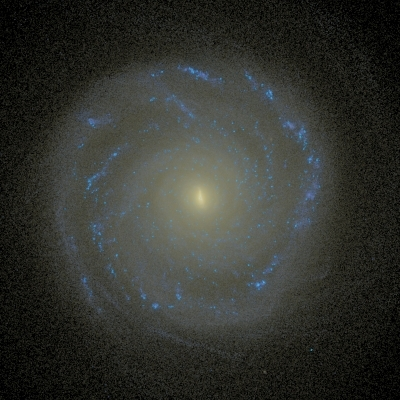
\includegraphics[angle=0]{h258_faceon_crop}}}
\caption[]{Face-on and edge-on Sunrise images of our GASOLINE galaxy, h258, which has an active, merger-rich history.}
\label{h258face} 
\end{figure}

\begin{figure}
\centerline{\resizebox{0.75\hsize}{!}{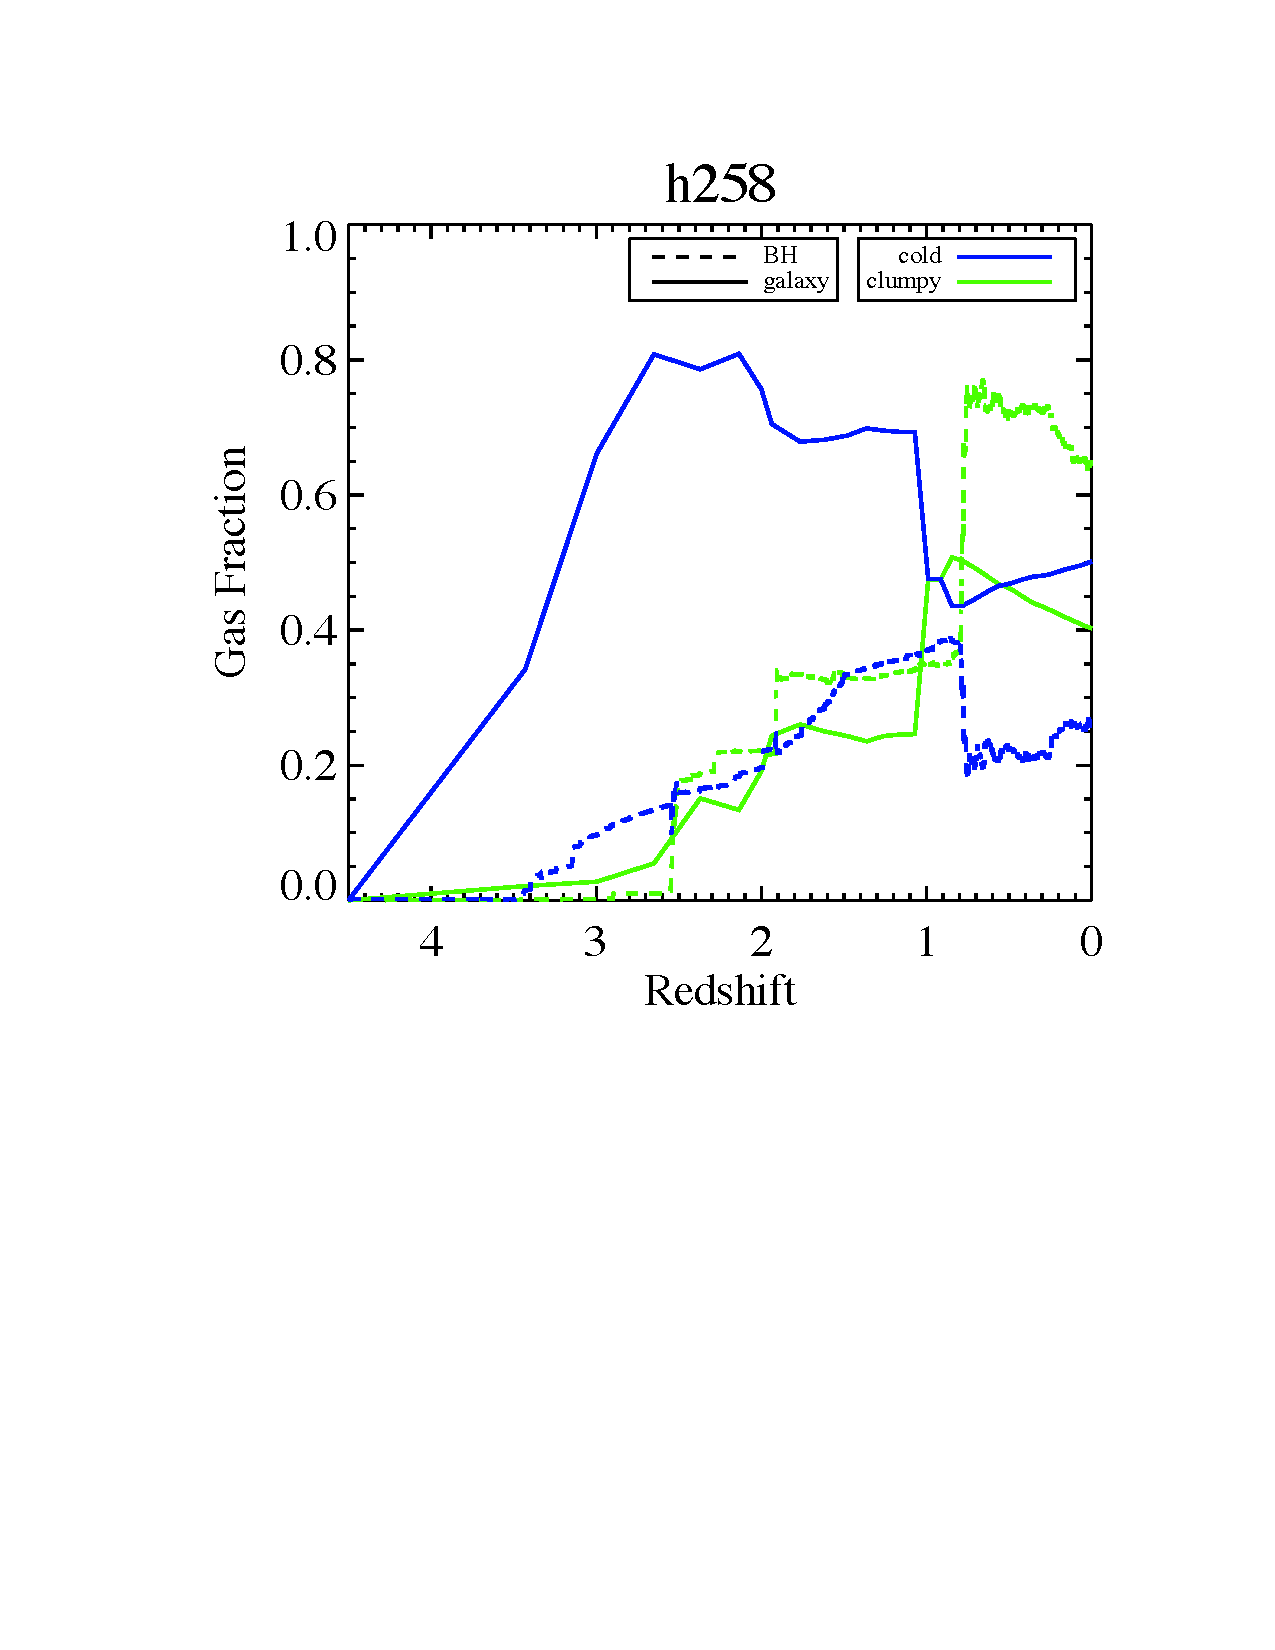
\includegraphics[angle=0]{h258numfraction_brightgreen}}}
\caption[]{Gas fraction across redshift for galaxy (solid lines) and central BH (dashed lines). Green lines signify gas fractions accreted via mergers and blue lines designate gas accreted via cold flow.}
\label{h258numfrac} 
\end{figure}

\begin{figure}
\centerline{\resizebox{0.75\hsize}{!}{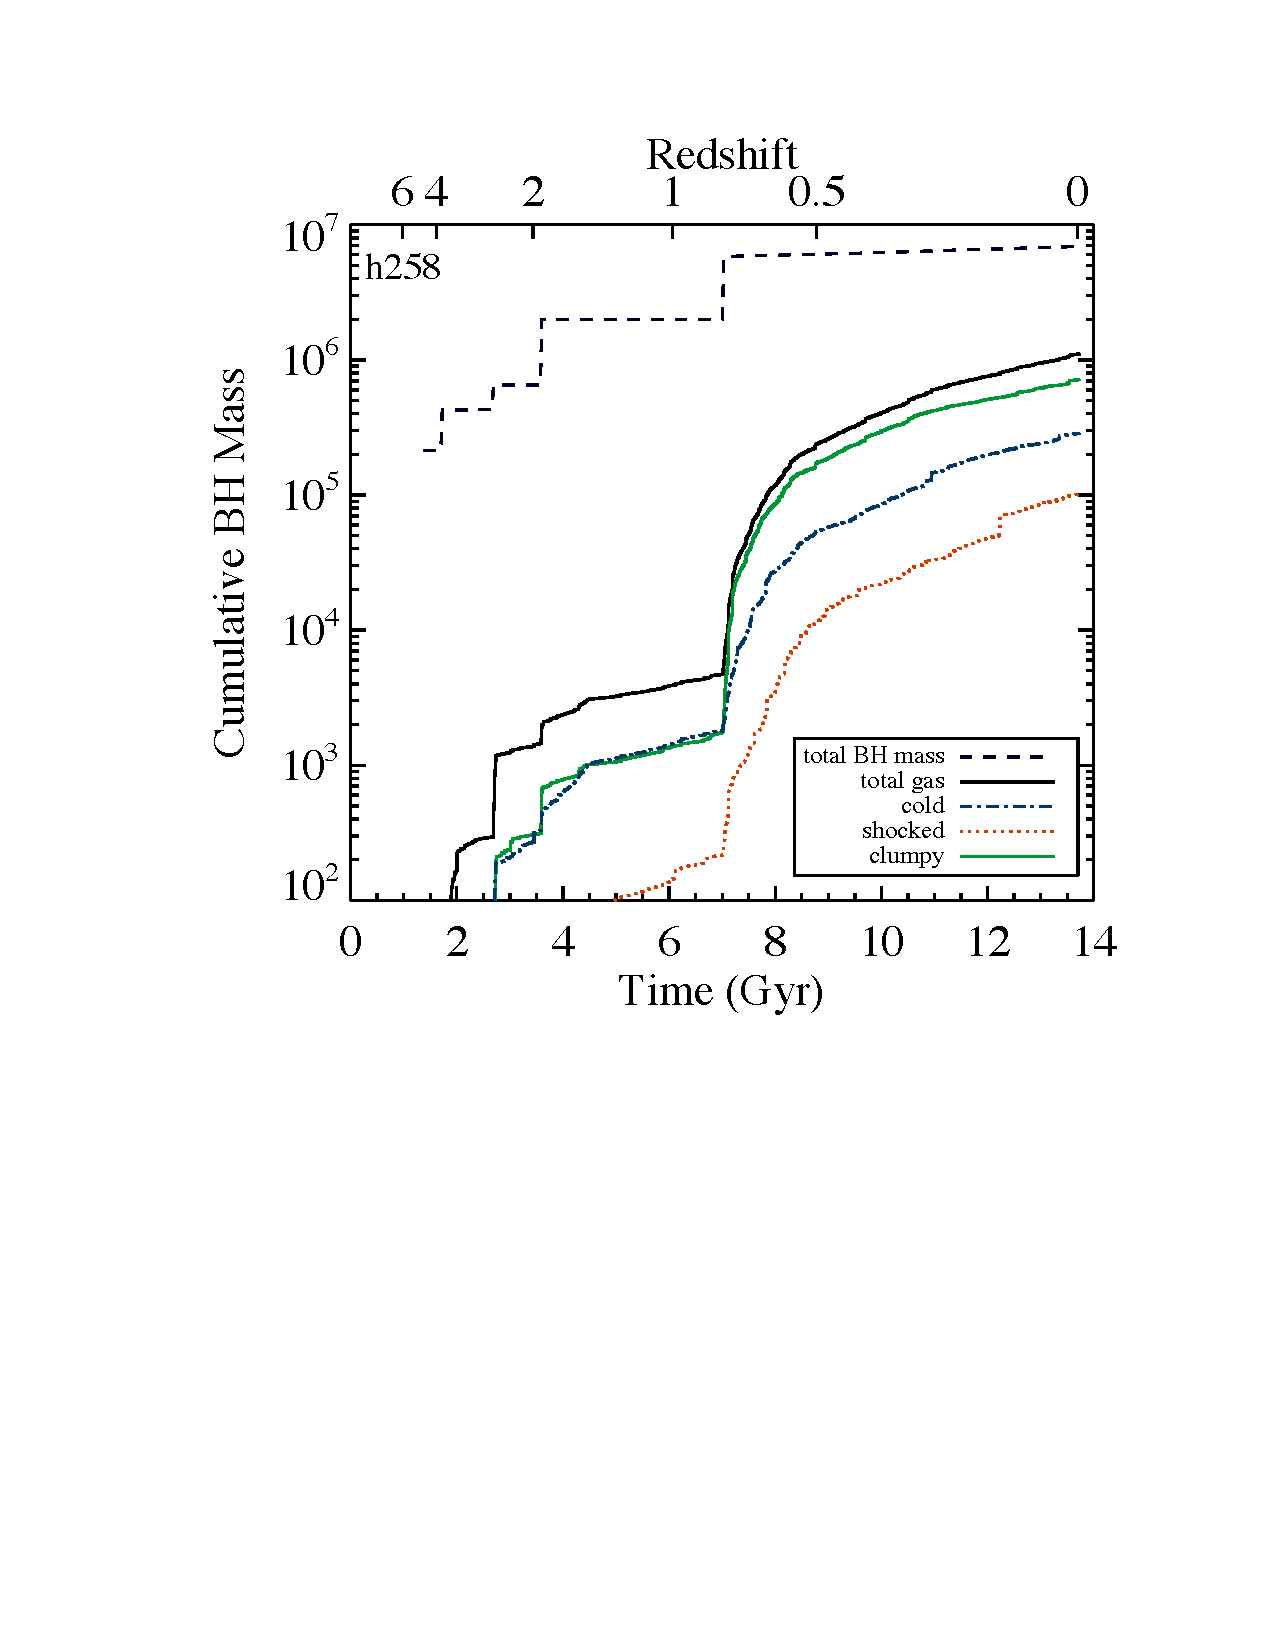
\includegraphics[angle=0]{h258_allmassgas_final}}}
\caption[]{The central BH’s cumulative mass as a function of time and redshift. The black dashed line indicates the total cumulative BH mass. The black solid line indicates the total gas mass. The blue dot-dashed line indicates the gas mass accreted via cold flows. The green solid line indicates the gas mass accreted through mergers. The red dashed line indicates gas mass that was shocked upon entry into the halo.}
\label{h258allmassgas} 
\end{figure}

\begin{figure}
\centerline{\resizebox{0.55\hsize}{!}{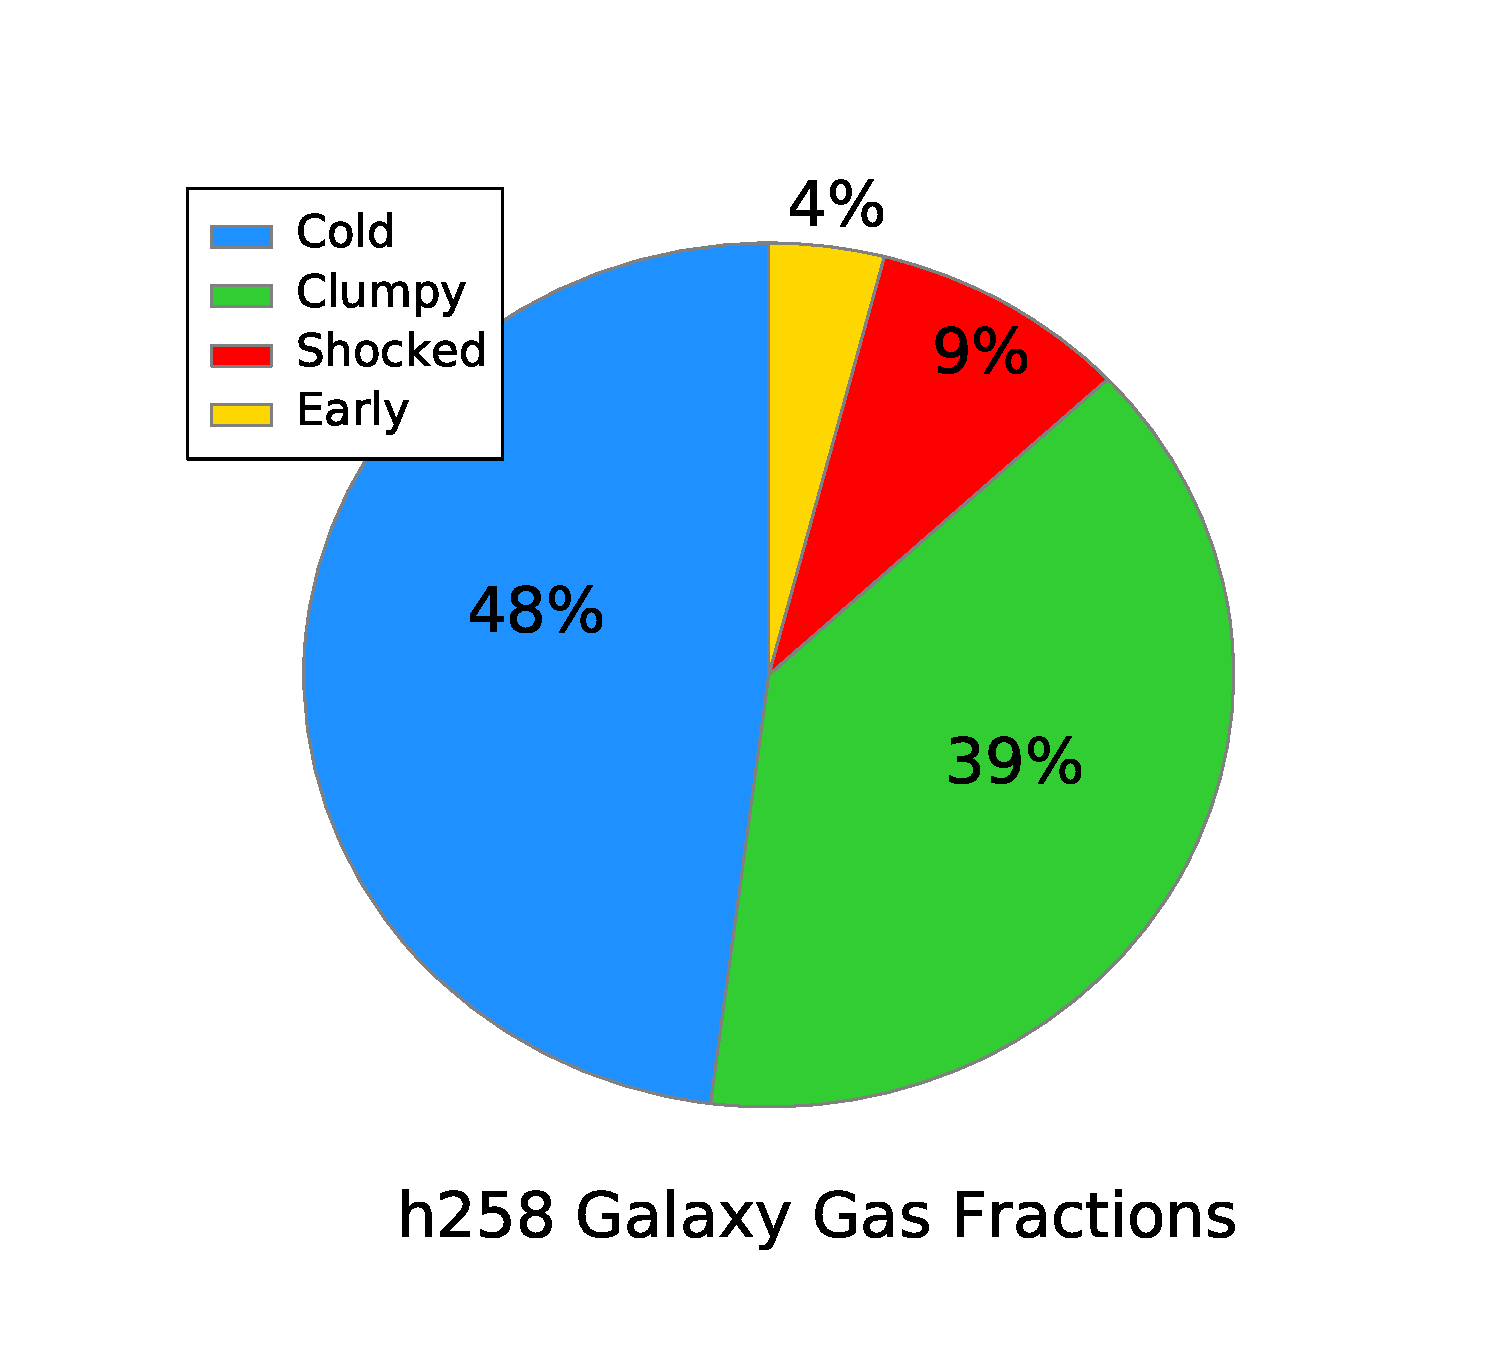
\includegraphics[angle=0]{PIE_h258galgasfrac_noexplode_realcolors}}}
\centerline{\resizebox{0.55\hsize}{!}{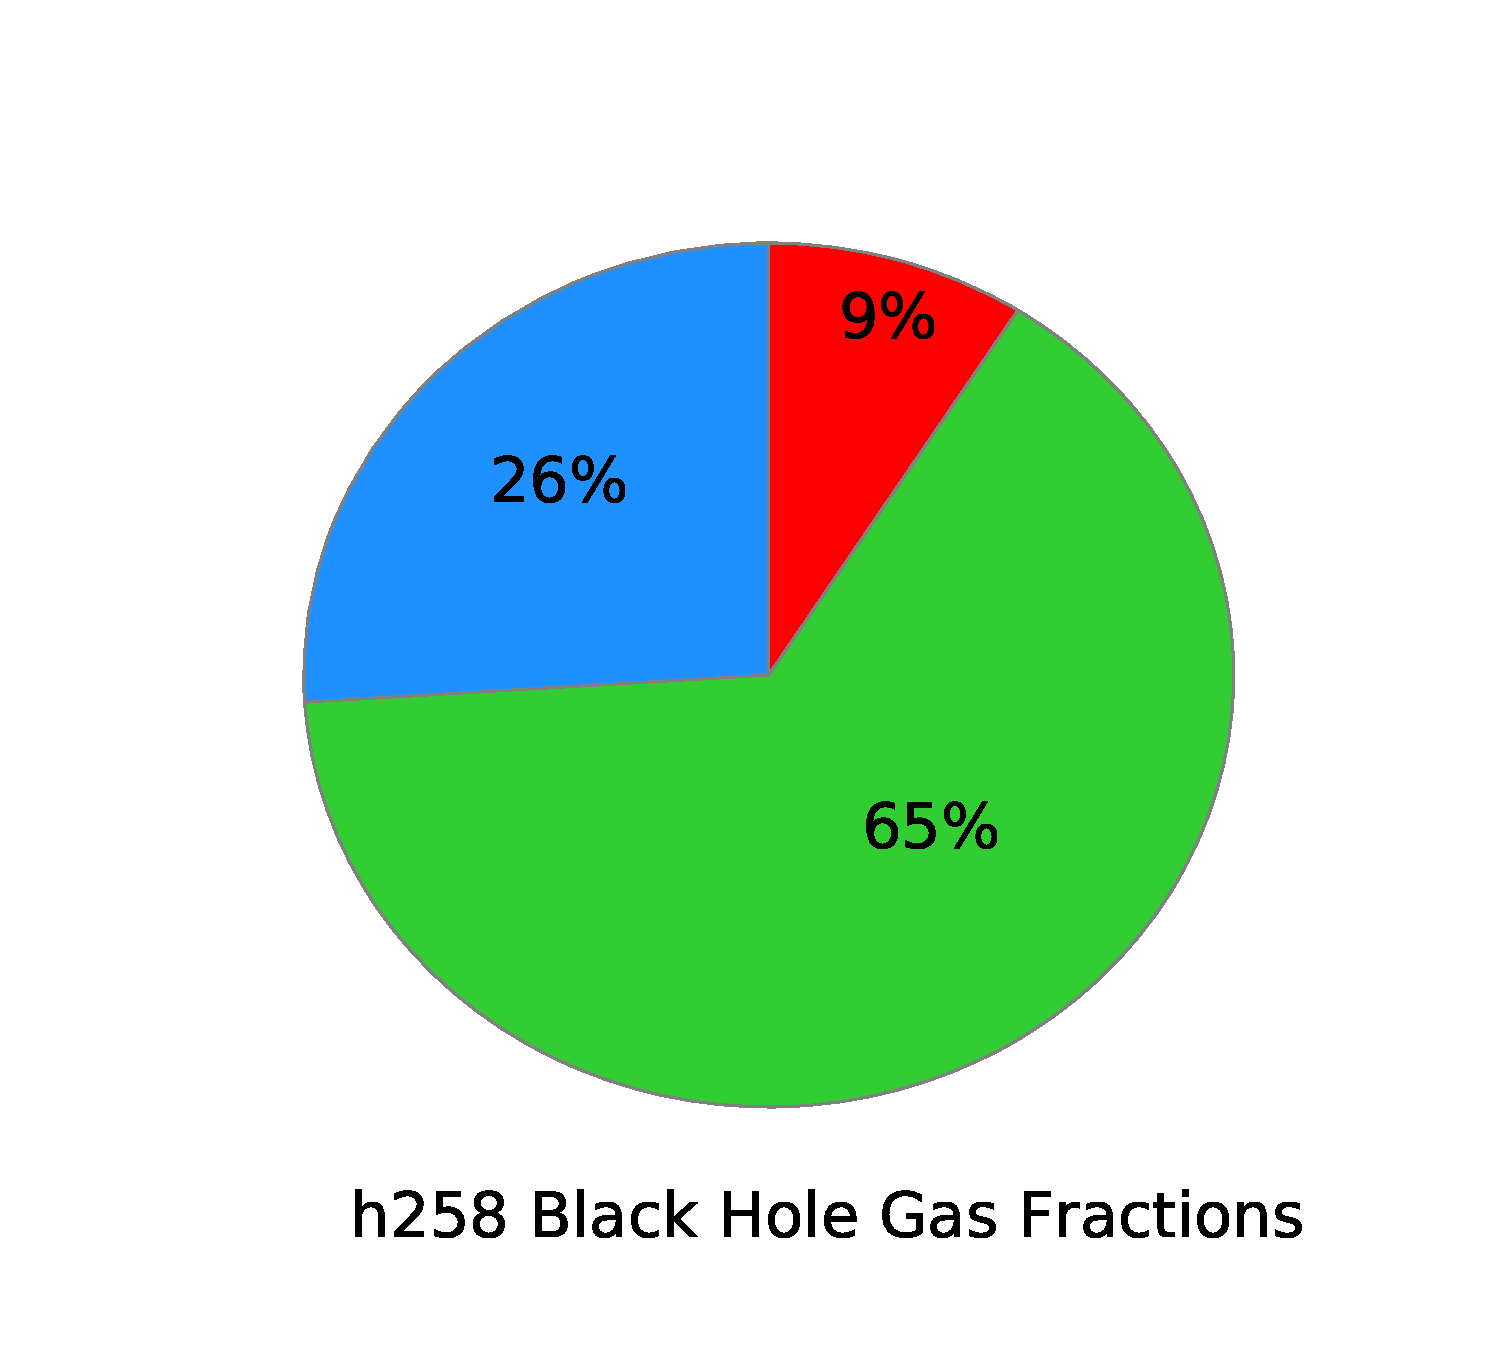
\includegraphics[angle=0]{PIE_h258bhgasfrac_noexplode_realcolors}}}
\caption[]{Gas fractions of the gas particles accreted in h258 by the main halo (above) and the SMBH (below), distinguished by type. Blue, green, and red distinguish gas gained through cold flows, gained through mergers, and gas shocked upon entry, respectively. Yellow indicates gas that existed within the main halo upon formation; this "early" gas is negligible (<1 \%) within the SMBH.}
\label{h258piefrac} 
\end{figure}

\begin{figure}
\centerline{\resizebox{0.75\hsize}{!}{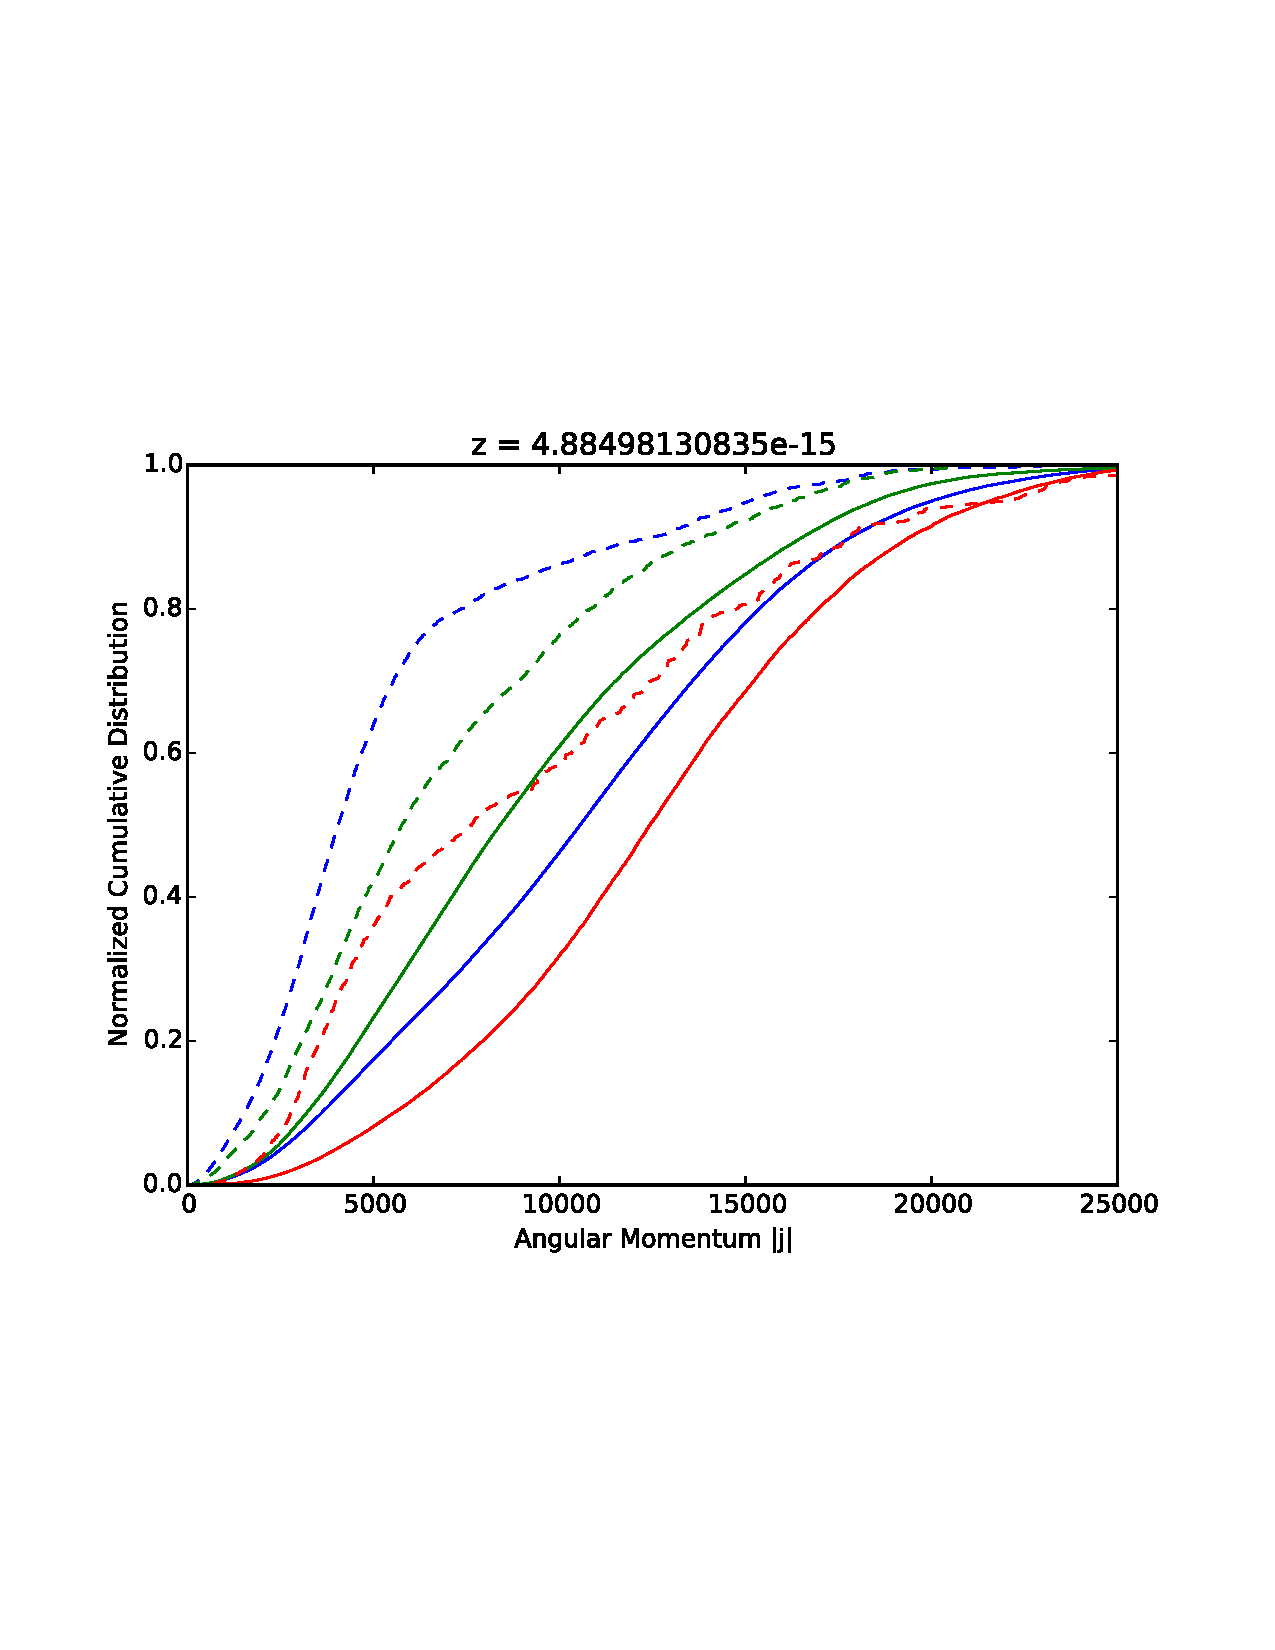
\includegraphics[angle=0]{h258_angmom_cumudist}}}
\caption[]{ Cumulative distribution of angular momentum of the gas particles accreted onto h258.  Gas particles accreted onto the main halo (solid lines) and central black hole (dashed lines). The green, blue, and red lines indicate clumpy, cold, and shocked gas, respectively.}
\label{h258angmom} 
\end{figure}

\begin{figure}
\centerline{\resizebox{0.75\hsize}{!}{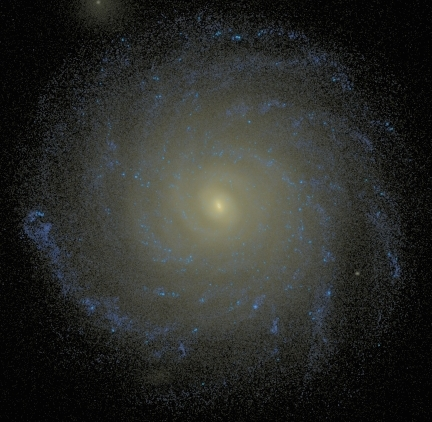
\includegraphics[angle=0]{h277_faceon}}}
\caption[]{Face-on and edge-on Sunrise images of our GASOLINE galaxy, h277, which has a quiescent, merger-quiet history.}
\label{h277face} 
\end{figure}

\begin{figure}
\centerline{\resizebox{0.75\hsize}{!}{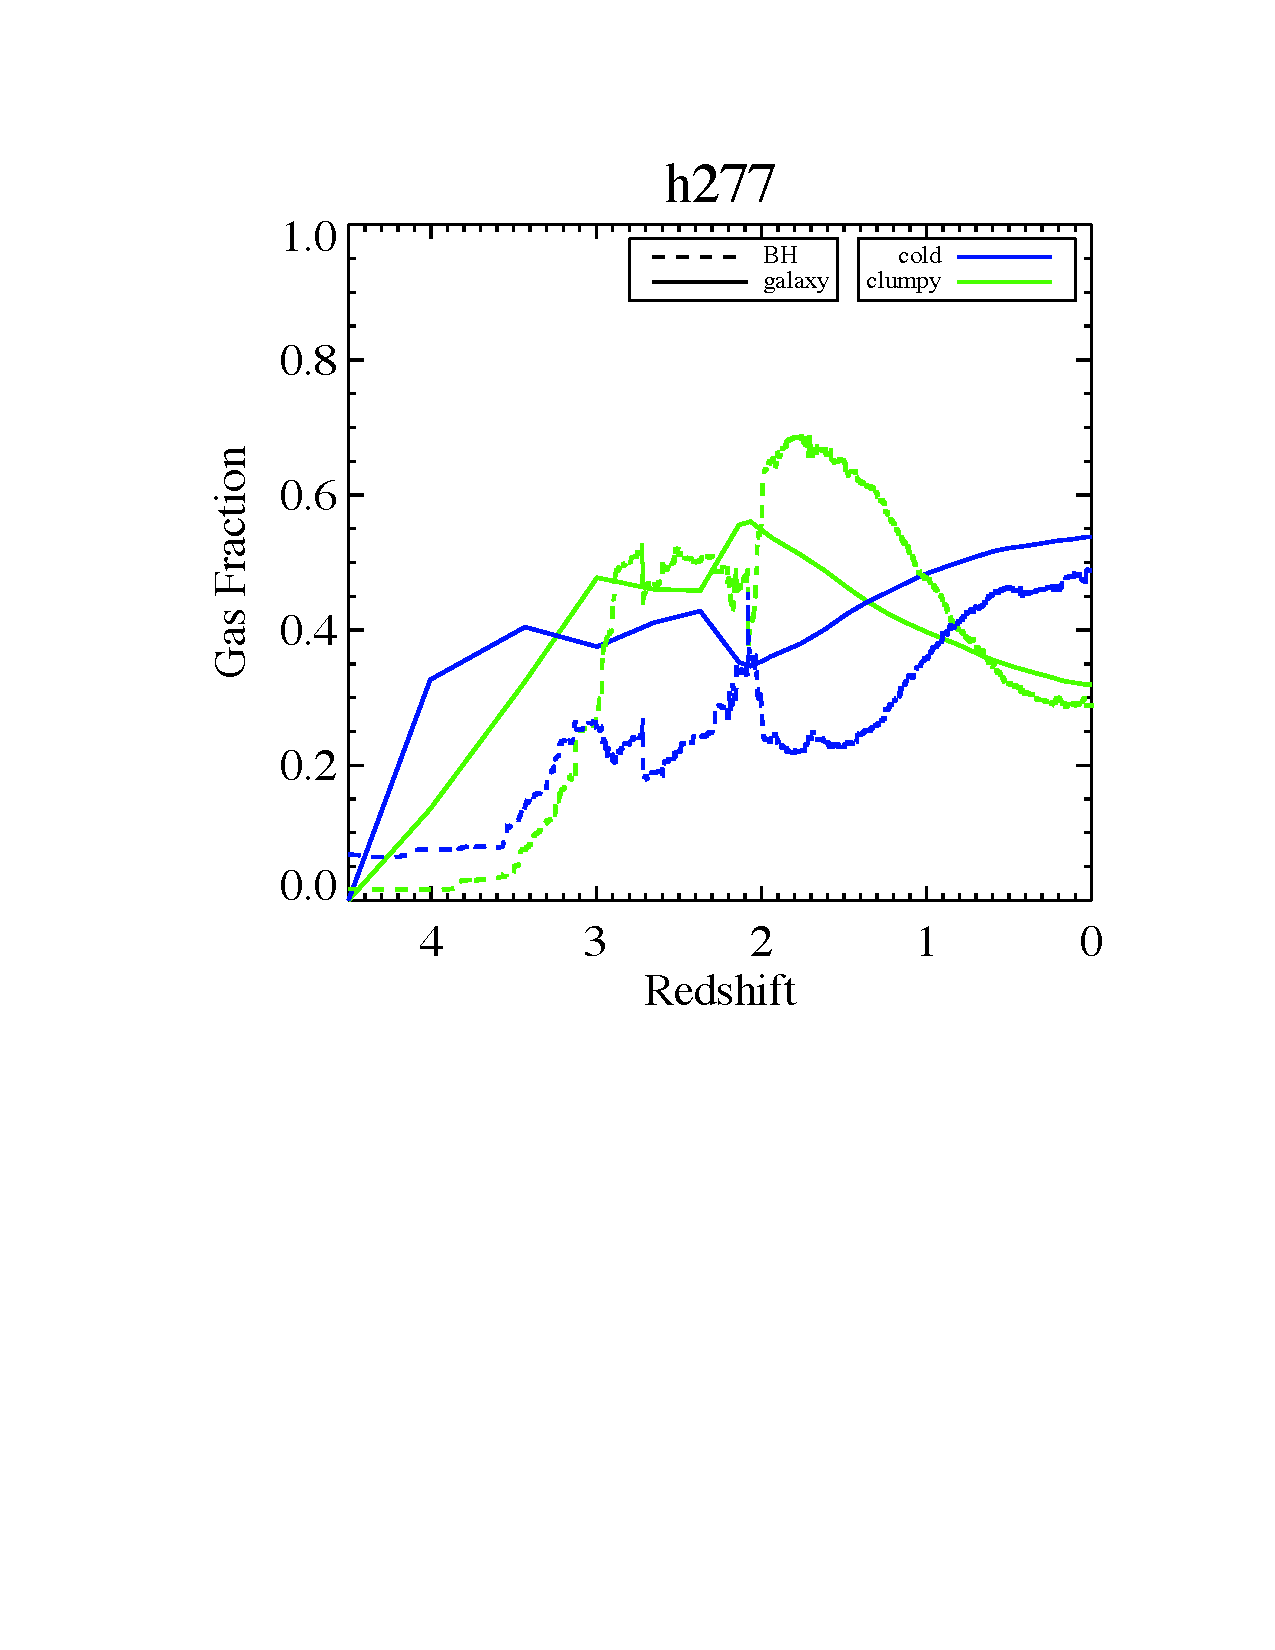
\includegraphics[angle=0]{h277numfraction_brightgreen}}}
\caption[]{Gas fraction across redshift for galaxy (solid lines) and central BH (dashed lines). Green lines signify gas fractions accreted via mergers and blue lines designate gas accreted via cold flow.}
\label{h277numfrac} 
\end{figure}

\begin{figure}
\centerline{\resizebox{0.75\hsize}{!}{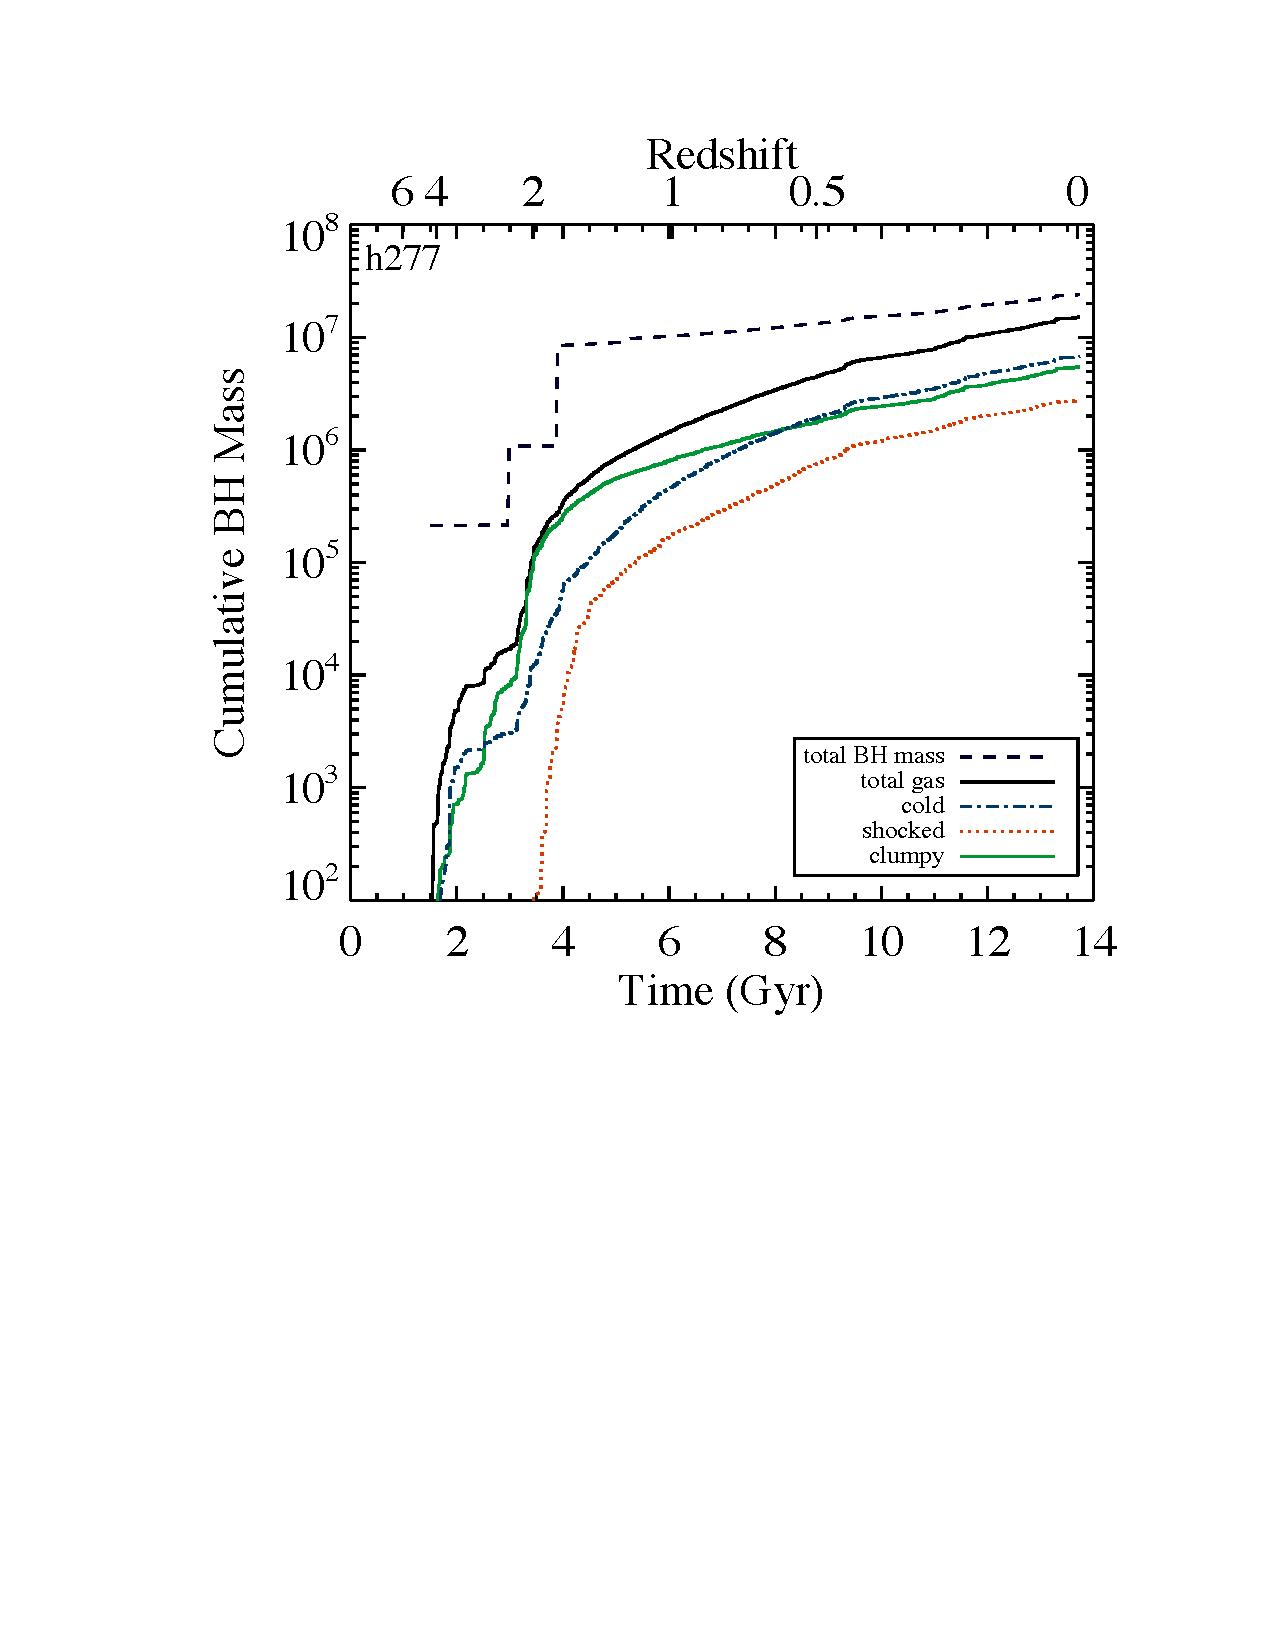
\includegraphics[angle=0]{h277_allmassgas_final}}}
\caption[]{The central BH’s cumulative mass as a function of time and redshift. The black dashed line indicates the total cumulative BH mass. The black solid line indicates the total gas mass. The blue dot-dashed line indicates the gas mass accreted via cold flows. The green solid line indicates the gas mass accreted through mergers. The red dashed line indicates gas mass that was shocked upon entry into the halo.}
\label{h277allmassgas} 
\end{figure}

\begin{figure}
\centerline{\resizebox{0.55\hsize}{!}{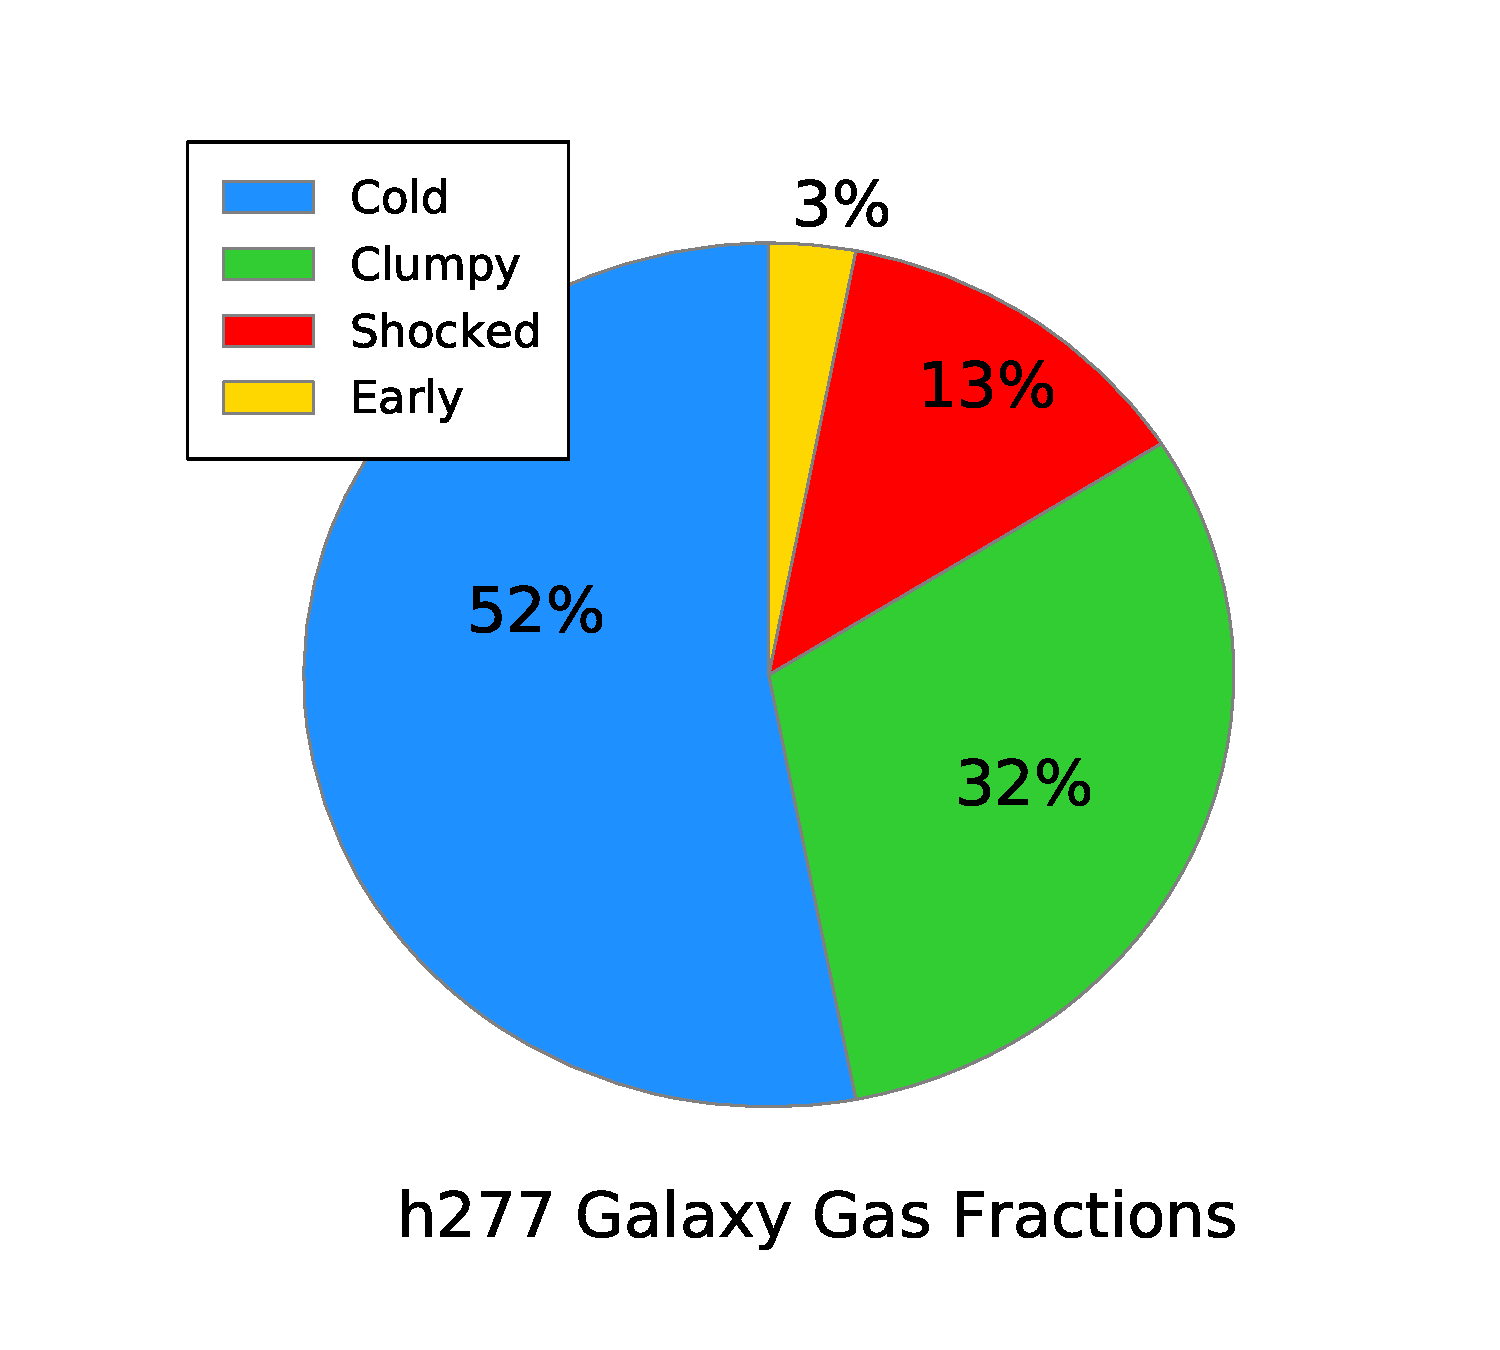
\includegraphics[angle=0]{PIE_h277galgasfrac_noexplode_realcolors}}}
\centerline{\resizebox{0.55\hsize}{!}{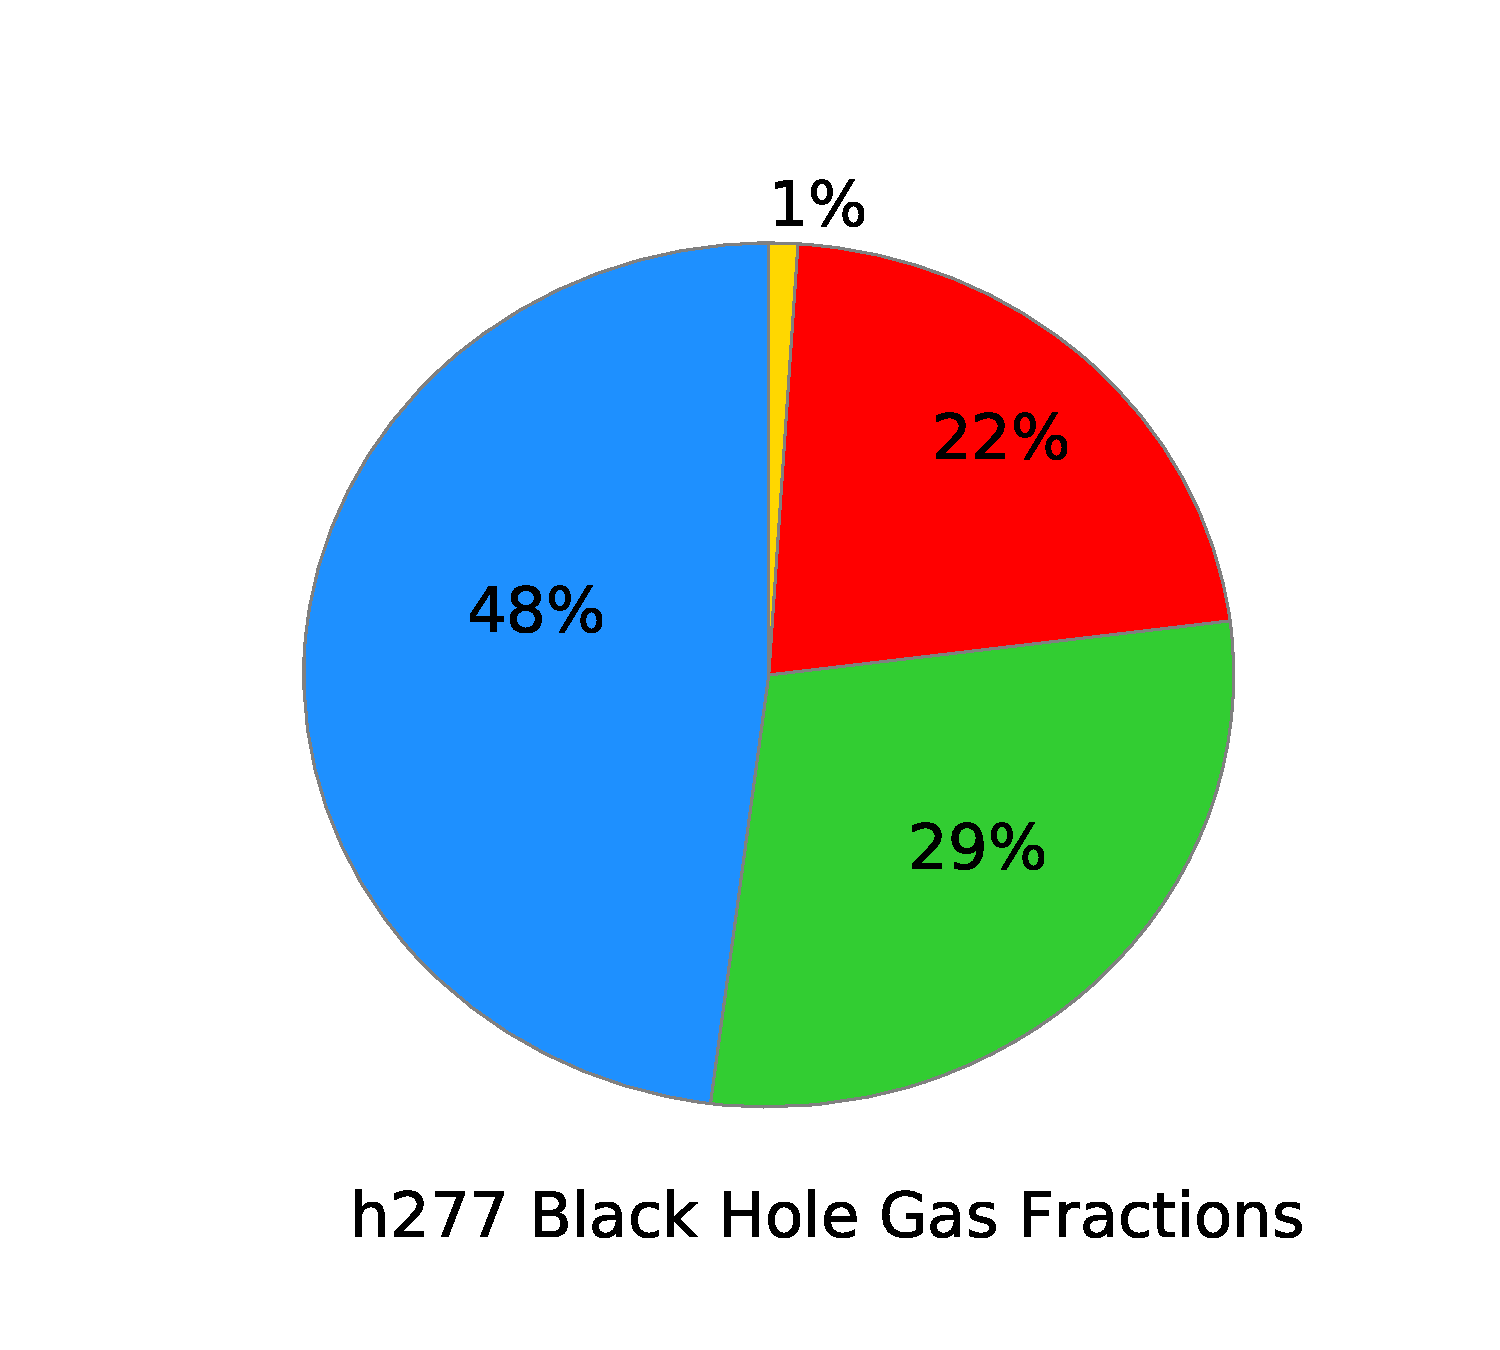
\includegraphics[angle=0]{PIE_h277bhgasfrac_noexplode_realcolors}}}
\caption[]{Gas fractions of the gas particles accreted in h258 by the main halo (above) and the SMBH (below), distinguished by type. Blue, green, and red distinguish gas gained through cold flows, gained through mergers, and gas shocked upon entry, respectively. Yellow indicates gas that existed within the main halo upon formation; this "early" gas is negligable (<1 \%) within the SMBH.}
\label{h277piefrac} 
\end{figure}

\begin{figure}
\centerline{\resizebox{0.75\hsize}{!}{\includegraphics[angle=0]{h277_angmom_cumudist_wrongaxis}}}
\caption[]{ Cumulative distribution of angular momentum of the gas particles accreted onto h277.  Gas particles accreted onto the main halo (solid lines) and central black hole (dashed lines). The green, blue, and red lines indicate clumpy, cold, and shocked gas, respectively.}
\label{h277angmom} 
\end{figure}


\bibliography{/Users/nicolesanchez/Documents/MENDELEY/MEND_bibtexfiles/Paper1.bib}


\end{document}

